\chapter{Bakgrunn}
\label{ch:background}

\section{Velferdsteknologi}
\citet{regjeringen_hagen} er en norsk offentlig utredning (NOU) om velferdsteknologi med tittelen «Innovasjon i omsorg».
Utredningen benytter følgende definisjon av velferdsteknologi:

\blockquote{
Med velferdsteknologi menes først og fremst
teknologisk assistanse som bidrar til økt trygghet,
sikkerhet, sosial deltakelse, mobilitet og
fysisk og kulturell aktivitet, og styrker den
enkeltes evne til å klare seg selv i hverdagen til
tross for sykdom og sosial, psykisk eller fysisk
nedsatt funksjonsevne. Velferdsteknologi kan
også fungere som teknologisk støtte til pårørende og
ellers bidra til å forbedre tilgjengelighet,
ressursutnyttelse og kvalitet på tjenestetilbudet.
Velferdsteknologiske løsninger kan i
mange tilfeller forebygge behov for tjenester
eller innleggelse i institusjon.
}

\begin{figure}
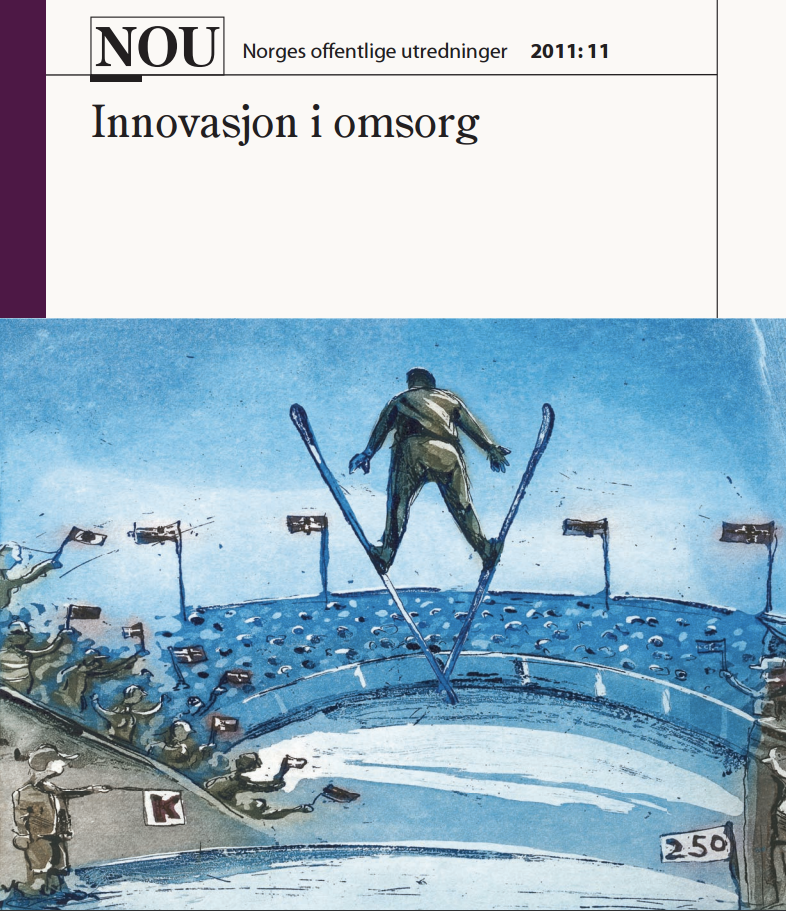
\includegraphics[width=0.85\textwidth,center]{fig/hagen}
\caption{Hagen-komiteen: Siden 2011 har det blitt hoppet over 250 meter i Vikersund, og verdensrekorden er nå 253,5 meter. }
\label{fig:hagen}
\end{figure}

\citet{regjeringen_hagen} anbefaler fem punkter for myndighetene å fokusere på i fremtiden:

\begin{enumerate}
    \item «Næromsorg» -- den andre samhandlingsreformen: mobiliser ressurser i samarbeid med
    lokalsamfunnet, det sosiale nettverket til pasienten og familien.
    \item «Teknoplan 2015» -- teknologistøtte til omsorg: bruk ny og eksisterende teknologi for å gi brukere
    bedre trygghet og muligheten til å bo hjemme og motta støtte.
    \item «Nye rom» -- fremtidens boligløsninger og nærmiljø: boliger og leiligheter må tilpasses eldre.
    \item Et nasjonalt program for kommunal innovasjon i omsorg: kommunene har hovedansvaret for omsorgstjenester,
    og myndighetene kan støtte kommunene med incentiver til nye løsninger.
    \item Omsorgsfeltet som næring: Norge kan være en ledende nasjon i utviklingen av nye omsorgsprodukter, og
    eksportere disse innovasjonene. Omsorgsfeltet åpnes opp for importering av eksportering av varer og tjenester.
\end{enumerate}

% @Todo: Spesielt teknoplan og nasjonalt program er interessant for denne oppgaven blabla (skrive noe mer om de to punktene).

Stortingsmeldingen «Morgendagens omsorg» bygger på arbeidet til \citet{regjeringen_hagen} \citep{morgendagens_omsorg}.
I denne meldingen legger regjeringen frem «Omsorgsplan 2020» som inkluderer et program for velferdsteknologi de neste årene.
Ett av initiativene i programmet er å bygge og etablere åpne velferdsteknologistandarder. Dette vil lette integreringen av nye
løsninger i privat og offentlig sektor. Andre initiativer er å utvikle og teste velferdsteknologiløsninger i kommunene,
bygge og dele kunnskap og lage modeller og rammeverk som andre kan bruke.

I revidert statsbudsjett for 2014 bevilget Stortinget penger til et nasjonalt velferdsteknologiprogram. De fem prioriterte
initativene i programmet er:

\begin{enumerate}
    \item Trygghet og mestring hjemme
    \item Avstandsoppfølging av personer med kroniske sykdommer
    \item mHelse
    \item Sosiale nettverk -- motvirke og redusere ensomhet blant eldre
    \item Bidra til økt aktivitet (inkl. fritidsaktiviteter) for barn og unge med nedsatt funksjonsevne
\end{enumerate}

\textquote{mHelse, eller personlige mobile helseløsninger, er å benytte mobilbaserte verktøy og helseapplikasjoner
(helse-apper) til helseformål}{.} % @TODO: kilde: https://ehelse.no/m-helse
De ulike initiativene går litt inn i hverandre. Avstandsoppfølging kan føre til mer trygghet og mestring hjemme
og ta i bruk mHelse. Avstandsoppfølging er dekket nærmere i delkapittel \ref{sec:remotemonitoring}.

\section{Avstandsoppfølging av kronisk syke}
\label{sec:remotemonitoring}
% @Todo: Chronic diseases are the most common causes of death and disability worldwide (med kilde).
\citet{rojahn2016remote} definerer avstandsoppfølging som \textquote{overvåking av en poliklinisk pasient
med en enhet som overfører data}{.}
I avstandsoppfølging følges pasienter opp i sitt eget hjem, og
målet med avstandsoppfølging er å unngå sykehusinnleggelse ved å oppdage forverringer tidlig og la
pasientene behandle sin egen sykdom. Innleggelse på sykehus koster 10 000 kr per døgn og er en stor utgift
for helsemyndighetene. % @Todo: kilde?

I følge \citet{austad2016sensorer}, kan kroniske sykdommer som KOLS, hjerte- og karsykdommer og diabetes
følges opp klinisk med noen få sensorer: vekt, blodtrykksmåler, pulsoksimeter og spirometer. Typiske
tegn på hjertesvikt kan være tungpusthet, vektforandring, hoste, hjertebank, hevelser i beina og
tretthet/tiltaksløshet \citep{ehelse_hjertesvikt}. % @TODO: http://nasjonalforeningen.no/hjerte-og-kar/ulike-hjertesykdommer/hjertesvikt/

% @Todo: Skrive noe om de ulike kommunene som tester ut avstandsoppfølging i Norge basert
% på nasjonalt program for velferdsteknologi.

% @Todo: Skrive noe om resultatene og evalueringen av avstandsoppfølging basert på rojahn,
% https://helsedirektoratet.no/nyheter/bedre-kvalitet-med-velferdsteknologi-i-helse-og-omsorgstjenestene
% http://www.ks.no/contentassets/7f30e3e8219b425484c885a3ee0dcd41/une-tangen.pdf

\section{Eldre pasienter og IT} 

\section{Tingenes internett (IoT)}
\citet{iot_legal} definerer tingenes internett som en
\textquote{fremvoksende global Internett-basert informasjonsarkitektur som
fasiliterer utvekslingen av varer og tjenester}{.} I denne definisjonen ligger det en
visjon av en verden knyttet sammen av objekter som kommuniserer med hverandre.

Andre definisjoner av \gls{iot} eksisterer avhengig av bransje. \citet{iot_harvard_smart} skriver
at tingenes internett ikke er en veldig god beskrivelse av den nye trenden med
sammenkoblete enheter: 
\textquote{Det som gjør smarte, tilkoblede produkter fundamentalt annerledes er ikke Internett,
men at «tingenes» natur endrer seg. Det er de nye mulighetene til smarte, tilkoblede produkter
og dataen de genererer som fører til en ny periode med konkurranse}{.}

Derfor introduserer de begrepet «smarte produkter» som består av tre elementer:

 \begin{itemize}
    \item Fysiske komponenter: de elektriske og mekaniske delene til produktet.
    \item «Smarte» komponenter: sensorer, prosessorer, programvare, operativsystem, lagring, brukergrenesnitt.
    \item Tilkoblingskomponenter: porter, antenner, protokoller som muliggjør kablede/trådløse tilkoblinger
    én-til-én, én-til-mange, mange-til-mange.
\end{itemize}

Smarte produkter introduserer en ny teknologistakk (figur \ref{fig:iot_harvard_smart}) med produkter koblet til
en produktsky. Produktskyen inkluderer et «Big Data»-databasesystem og regel- og analysemotor for å håndtere
forretningslogikk på en effektiv måte, og utnytte og analysere all informasjonen fra produktene.
Disse smarte, tilkoblede produktene har fire egenskaper som bygger på hverandre: Overvåking, kontroll,
optimalisering og autonomi. Tesla er et eksempel på et smart produkt som kombinerer overvåking, kontroll og
optimalisering for å oppnå autonomi. Bilen diagnoserer seg selv, og oppdaterer seg selv automatisk uten
at den må på verksted.

\citet{iot_harvard_smartcompanies} antyder at smarte, tilkoblede produkter endrer selskaper også, ved
å endre hvert steg i verdikjeden. Utnyttelse av data blir mer viktig, og produktdesign er ikke bare noe
mekanisk, men et tverrfaglig samarbeid der programvareutvikling vil spille en større rolle. 

\begin{figure}
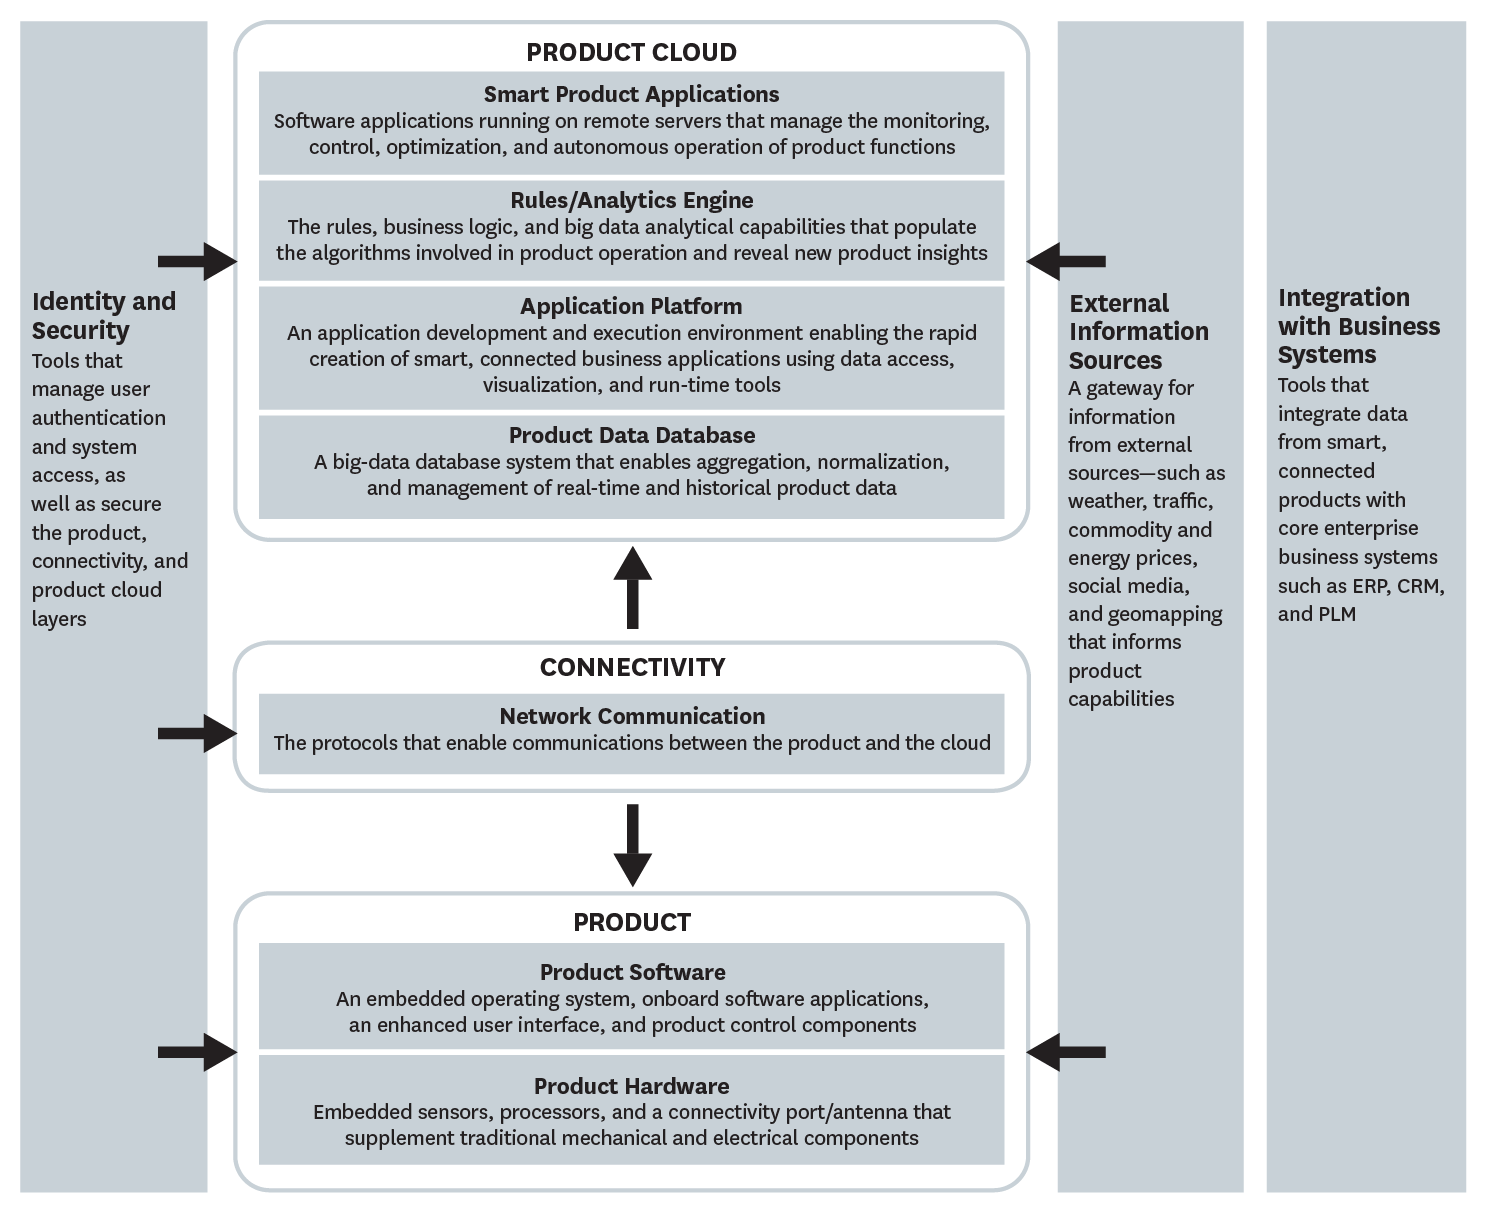
\includegraphics[width=1.1\textwidth,center]{fig/harvard_technology}
\caption{Den nye teknologistakken \citep{iot_harvard_smart}.}
\label{fig:iot_harvard_smart}
\end{figure}

\begin{figure}
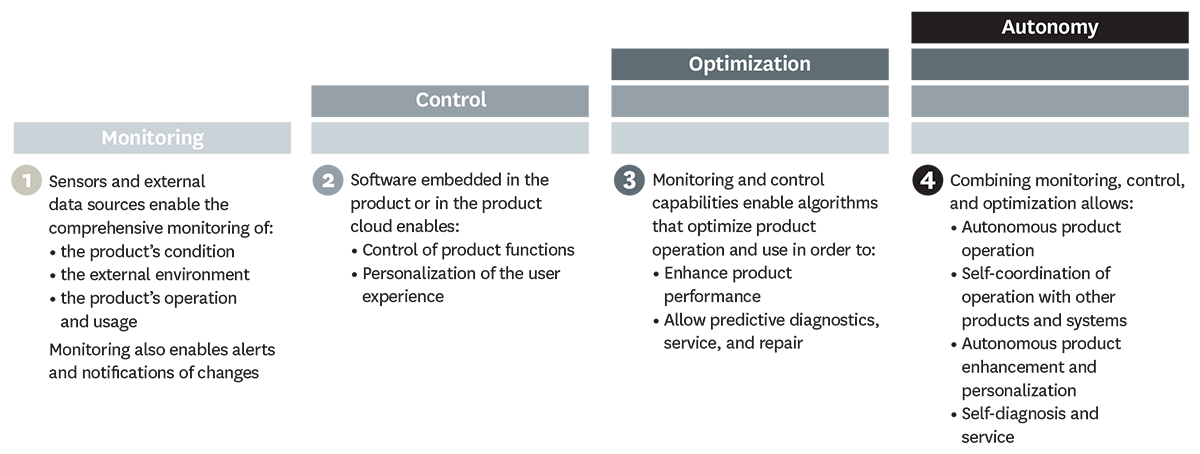
\includegraphics[width=1.1\textwidth,center]{fig/harvard_capabilities}
\caption{Egenskapene til smarte produkter \citep{iot_harvard_smart}.}
\label{fig:iot_harvard_capabilities}
\end{figure}


\subsection{Sikkerhet i tingenes internett}
Eksperter har kommet med innvendinger når det gjelder sikkerhetsmodellen til \gls{iot}.
21. oktober 2017 ble Internett-kjerneinfrastrukturselskapet \textit{Dyn} angrepet av flere millioner
små enheter (hovedsaklig rutere og kameraer) med lav grad av sikkerhet \citep{iot_attack_ddos}.
Dette påvirket flere store nettsider som Twitter, Spotify og PayPal. Rutere og webkameraer leveres
ofte med standardpassord som brukere ikke endrer selv. I tillegg til dette kan flere vanlige
porter som 22 (SSH), 80 (HTTP) og 23 (Telnet) være helt åpne mot omverdenen \citep{iot_mirai_botnet}.

\citet{iot_schneier_regulation} oppfordrer myndighetene til å pålegge restriksjoner på \gls{iot}.
Han argumenterer for at markedene selv ikke klarer å beskytte sikkerheten til forbrukerne.
Forbrukerne bryr seg ikke, produsentene bryr seg ikke og produktene kan aldri patches
etter de er solgt og levert. Denne diskusjonen om reguleringer må gjøres før det skjer
en \gls{iot}-katastrofe, mener Schneier. % @Todo: en iot-katastrofe where feelings are heated?


\section{Tingenes internett i velferdsteknologi}
Personal Connected Health Alliance (PCHA) publiserer Continua-designretningslinjene hvert år,
et åpent rammeverk for ende-til-ende-kompabilitet i personlige, tilkoblede helseenheter og helsesystemer \citep{continua_guidelines}.
En oversikt av Continua-rammeverket kan finnes i figur \ref{fig:continua}. Personlige enheter kommuniserer med
protokoller som Bluetooth eller Zigbee til en hub (Personal Area Network), og denne huben sender informasjonen
videre til et telehelse-servicesenter. Derfra kan dataen overføres til helseregisteret.

Som en del av «Omsorgsplan 2020» og nasjonalt program for velferdsteknologi, bestemte regjeringen
i slutten av 2014 at Continua-rammeverket skal være grunnlaget for alle velferdsteknologiløsninger i Norge.
Dette var også anbefalingen til Helsedirektoratet --
å standardisere på ett rammeverk sikrer at ulike løsninger virker godt sammen \citep{regjeringen_continua}.

\begin{figure}
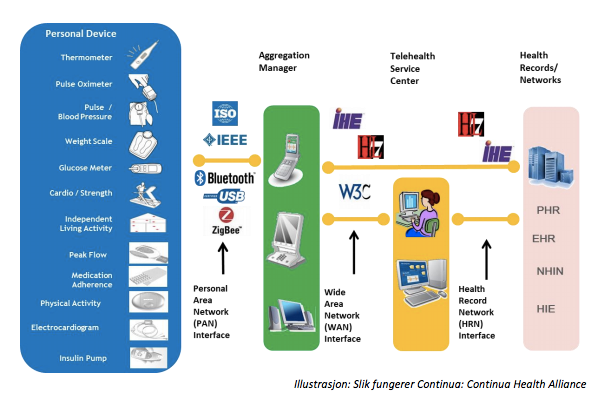
\includegraphics[width=0.9\textwidth,center]{fig/continua}
\caption{Oversikt over Continua-rammeverket}
\label{fig:continua}
\end{figure}
